% 默认页面大小 4:3
\documentclass[10pt]{ctexbeamer}
% 页面大小 16:10
% \documentclass[10pt, aspectratio=1610]{ctexbeamer}
% 页面大小 16:9
% \documentclass[10pt, aspectratio=169]{ctexbeamer}
% 页面大小 14:9
% \documentclass[10pt, aspectratio=149]{ctexbeamer}
% 页面大小 1.41:1
% \documentclass[10pt, aspectratio=141]{ctexbeamer}
% 页面大小 5:4
% \documentclass[10pt, aspectratio=54]{ctexbeamer}
% 页面大小 3:2
% \documentclass[10pt, aspectratio=32]{ctexbeamer}
\usepackage[export]{adjustbox}
\usetheme[logo=UCAS]{ucas}
% logo 的选项: CAS, UCAS
% sublogo 的选项: AMSS, AMSS2018, UCAS

% 引入参考文献列表的 .bib 文件, 使用 GB/T 7714-2015 的文献著录规则.
\usepackage[backend=biber, style=gb7714-2015]{biblatex}
\usepackage{svg}
\usepackage{wrapfig}
\addbibresource{ref.bib}

\title[组会汇报]{GPU-Initiated On-Demand High-Throughput Storage Access in the BaM System Architecture}
\subtitle{论文分享}
\author[D.\,Chen]{\href{chende23@mails.ucas.ac.cn}{陈德}}
% \institute[NJC, CAS]{中国科学院数学与系统科学研究院}
\date[\today]{\today}
% \subject{展示主题}
% \keywords{展示, 关键词}

\begin{document}

\begin{frame}[plain]
  \maketitle
\end{frame}

\begin{frame}[t]
  \frametitle{目录}
  \tableofcontents
\end{frame}

\section[1.Introduction]{1. Introduction}\label{sec:1}
\subsection[1.1 General]{1.1 总体介绍}\label{subsec:1-1}

\begin{frame}[t]
  \frametitle{1.Introduction}
  % \framesubtitle{幻灯片副标题}
  % 平凡格式\quad\structure{浅灰格式}\quad\alert{强调格式}
  % \begin{itemize}
  %   \item 第一级文本内容
  %   \item 若该行文本内容十分长长长长长长长长长则会被强制换行
  %     这里也可以包含\alert{需要强调的文本}
  %     \begin{itemize}
  %       \item 第二级文本内容
  %         \begin{itemize}
  %           \item 第三级文本内容
  %         \end{itemize}
  %         \alert{\item 第二级强调的文本内容}
  %     \end{itemize}
  % \end{itemize}
  %换行
  \begin{itemize}
    \item GPU已经是HPC和机器学习应用最主要的设备之一
    \begin{itemize}
      \item Graph and data analytics
      \item Graph neural networks(GNNs)
      \item Recommendation systems
    \end{itemize}
  \item 数据集大小增长迅速,从数十GB到数TB,并且在可见的未来会继续增长
  \end{itemize}

  \vfill
  \pause% 动态展示以下内容
  传统上,GPU依赖于主机CPU来启动对数据存储的访问,这对于具有已知数据访问模式的GPU应用来说是合适的。然而,随着图分析、数据分析、推荐系统或图神经网络等新兴应用的出现,这些应用需要更细粒度的、依赖于数据的存储访问,而CPU启动的存储访问由于高CPU-GPU同步开销、I/O流量放大和长的CPU处理延迟而变得不适合。
  % \begin{enumerate}
  %   \item 带序号的文本内容
  %     \begin{enumerate}
  %       \item 第二级文本内容且包含数学公式
  %         \[\int^{\infty}_{-\infty}e^{-x^2}dx = \sqrt{\pi}\]
  %     \end{enumerate}
  % \end{enumerate}
\end{frame}

\begin{frame}
  \frametitle{1.1 总体介绍}


  该论文提出了一种名为BaM(Big accelerator Memory)的原型系统,是第一个以加速器为中心的方法,GPU 可以对存储的数据(无论是内存还是存储)创建按需访问,而无需依赖 CPU 来启动或触发访问。
  
  \begin{itemize}
    \item 构建了一个高度并发的提交/完成协议队列的库,实现对存储的按需、高吞吐量、细粒度访问
    \item 提供了高吞吐量且可扩展的软件定义缓存和相应的API,来提高对局部性的利用
    \item 构建并评估 GPU 的原型设计,以便以经济高效的方式访问海量存储数据。
  \end{itemize}

\end{frame}

% \subsection[第 2 节缩写标题]{第 2 节标题}\label{subsec:1-2}

% \begin{frame}[t]
%   \frametitle{文本区块}
%   将文本放入区块内
%   \begin{block}{普通区块}
%     见 \citeauthor{guowei2019ucasbeamer}(\citeyear{guowei2019ucasbeamer}) 提供的模板
%   \end{block}
%   \begin{exampleblock}{示例区块}
%     \red{红色}
%   \end{exampleblock}
%   \begin{alertblock}{强调区块}
%     \green{绿色}
%   \end{alertblock}
%   脚注\footnote{\url{https://github.com/icgw/ucas-beamer}}
% \end{frame}



% \subsection[第 3 节缩写标题(虽然是缩写也可以很长长长长长长)]{第 3 节标题}\label{subsec:1-3}

% \begin{frame}[t]
%   \frametitle{表格}
%   \begin{table}
%     \begin{tabular}{lcl}\toprule
%       姓名   & 出生年份 & 母校 (本科)  \\ \midrule
%       陶哲轩 & 1975     & 弗林德斯大学 \\
%       张益唐 & 1955     & 北京大学     \\
%       丘成桐 & 1949     & 香港中文大学 \\ \bottomrule
%     \end{tabular}
%     \caption{二十一世纪的数学家}
%   \end{table}
% \end{frame}

% \begin{frame}[t]
%   \frametitle{引用}
%   \begin{theorem}[\citeauthor{graham1989concrete}\citeyear{graham1989concrete}]\label{thm1}
%     \[\textbf{具体 (\red{Concrete})} = \textbf{连续 (\red{Con}tinuous)} + \textbf{离散 (Dis\red{crete})}\]
%   \end{theorem}
%   \vfill
%   \begin{proof}
%     证明过程.
%   \end{proof}
%   引用定理~\ref{thm1}.
%   \blfootnote{\printbibliography[heading=none,keyword={concrete}]}
% \end{frame}

\section[2.Background]{2.Background}\label{sec:2}
\subsection{2.1 PCIe介绍}\label{sec:2-1}
% \makeatletter
% \begin{frame}[t]
%   \frametitle{自定义字体大小}
%   \begin{center}
%     \begin{tabular}{ll}
%       \Huge  $\backslash$Huge                & \Huge \structure{24.88 pt}     \\
%       \huge  $\backslash$huge                & \huge \structure{20.74 pt}     \\
%       \LARGE $\backslash$LARGE               & \LARGE \structure{17.28 pt}    \\
%       \Large $\backslash$Large               & \Large \structure{14.4 pt}     \\
%       \large $\backslash$large               & \large \structure{12 pt}       \\
%       \normalsize $\backslash$normalsize     & \normalsize \structure{10 pt}  \\
%       \small $\backslash$small               & \small \structure{9 pt}        \\
%       \footnotesize $\backslash$footnotesize & \footnotesize \structure{8 pt} \\
%       \scriptsize $\backslash$scriptsize     & \scriptsize \structure{7 pt}   \\
%       \tiny $\backslash$tiny                 & \tiny \structure{5 pt}
%     \end{tabular}
%   \end{center}
% \end{frame}
% \makeatother

\begin{frame}
  \frametitle{2.1 PCIe介绍}
  PCIe是以包(Packet)为单位传输数据的。和计算机网络类似,其协议也是分层的。其协议栈主要分为三层:物理层(Physical Layer),数据链路层(Data Link Layer)和事务层(Transaction Layer)
  \begin{itemize}
    \item 事务层,这一层定义了所有和用户相关的PCIe的操作。PCIe有4种事务:内存事务、IO事务、配置事务、消息事务。
    \item 数据链路层,对于上层发送的事务,负责保证事务消息能正确的传输到目的地。
    \item 物理层,主要将数据转换为易于介质传输的电信号,并发送出去,或者将接收到的转换后的信号,转变为上层能处理的数据包。
  \end{itemize}
\end{frame}
\begin{frame}[t]
  \frametitle{2.1 PCIe介绍}
  Root Complex是整个PCIe设备树的根节点,CPU通过它与PCIe的总线相连,并最终连接到所有的PCIe设备上。
  PCIe的总线并不是我们传统意义上共享线路的总线(Bus),而是一个点对点的网络,我们如果把PCI比喻成网络中的集线器(Hub),那么PCIe对应的就是交换机了。
  \begin{figure}
    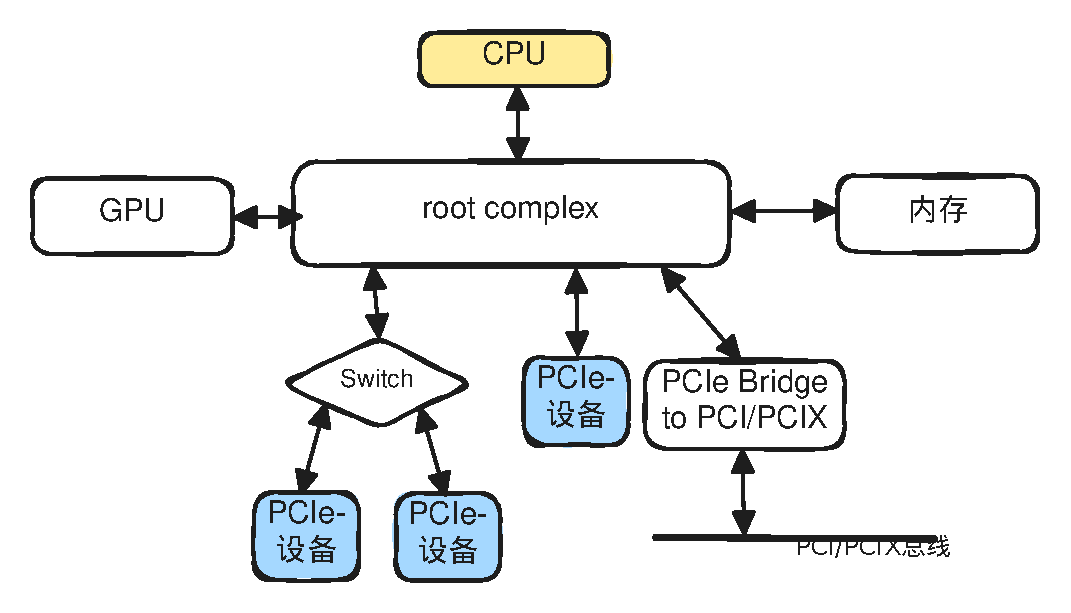
\includegraphics[width=.5\textwidth, height=.5\textheight, keepaspectratio]{images/pcie.eps}
  \end{figure}

\end{frame}

\subsection{2.2 NVMe介绍}\label{sec:2-2}
\begin{frame}
  \frametitle{2.2 NVMe介绍}
  NVMe(Non-Volatile Memory Express)协议是一种专为使用非易失性存储器(如固态硬盘SSD)而设计的高性能存储接口协议。
  NVMe协议制定了主机与SSD之间通过命令来通信。
  \begin{itemize}
    \item Admin命令,用于管理和控制SSD设备
    \item I/O命令,用于主机和SSD之间传输数据
  \end{itemize}
  \begin{figure}
    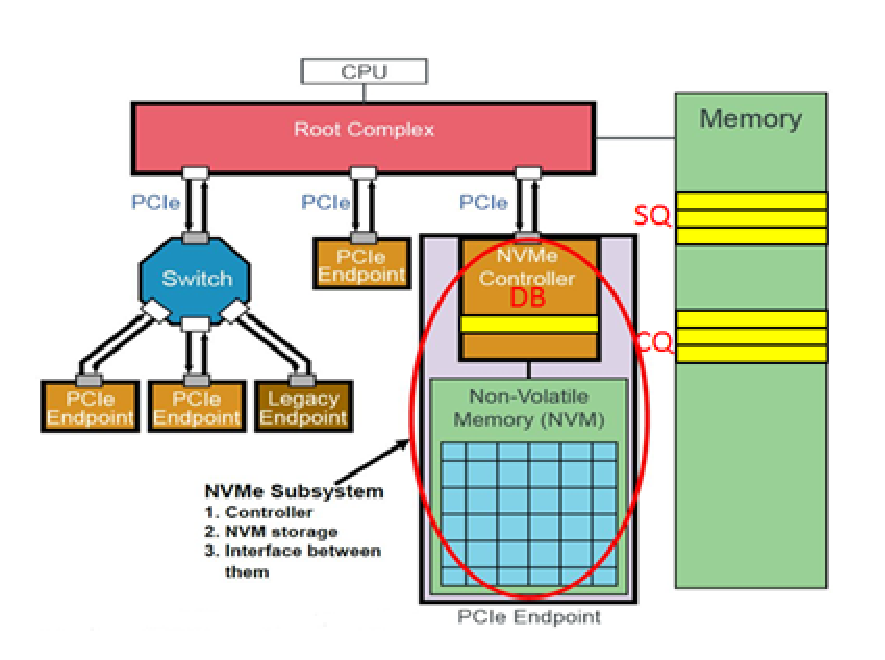
\includegraphics[width=.5\textwidth, height=.5\textheight, keepaspectratio]{images/nvme.eps}
  \end{figure}
\end{frame}

\begin{frame}
  SQ,CQ,DB是NVMe协议中的三个重要概念:
  \begin{itemize}
    \item SQ(Submission Queue):主机将命令写入SQ,SSD从SQ中取出命令执行
    \item CQ(Completion Queue):SSD将命令执行结果写入CQ,主机从CQ中取出命令执行结果
    \item DB(Doorbell register):位于SSD控制器内部,用于通知SSD有新的命令需要执行
  \end{itemize}
  \begin{figure}
    \includegraphics[width=.7\textwidth, height=.7\textheight, keepaspectratio]{images/nvme-queues.eps}
  \end{figure}
\end{frame}

\begin{frame}
  下图展示了NVMe一次完整处理指令的流程,共八步:
  \begin{enumerate}
    \item Host将指令写到SQ;
    \item Host写DB,通知SSD取指令;
    \item SSD收到通知,从SQ中取走指令;
    \item SSD执行指令;
    \item 指令执行完成,SSD往CQ写入指令执行结果;
    \item SSD通知Host指令执行完成;
    \item Host收到通知,处理CQ,查看指令完成状态;
    \item Host处理完CQ中的指令执行结果,通过DB回复SSD
  \end{enumerate}
  \begin{figure}
    \includegraphics[width=.5\textwidth, height=.5\textheight, keepaspectratio]{images/nvme-proc.eps}
  \end{figure}
  
\end{frame}

\section[3.Architecture]{3.BaM System and Architecture}\label{sec:3}
\subsection{3.1 BaM System}\label{sec:3-1}
\begin{frame}
  \frametitle{3.1 BaM 总体架构}
  BaM(Big accelerator Memory)系统的总体架构旨在提供一个高效、细粒度的存储访问机制,允许GPU(图形处理单元)线程直接、按需地访问存储设备上的数据。BaM的设计目标是提高存储访问性能,同时减少CPU(中央处理单元)的介入,从而降低CPU-GPU同步开销和操作系统内核的软件瓶颈。
  \begin{figure}
    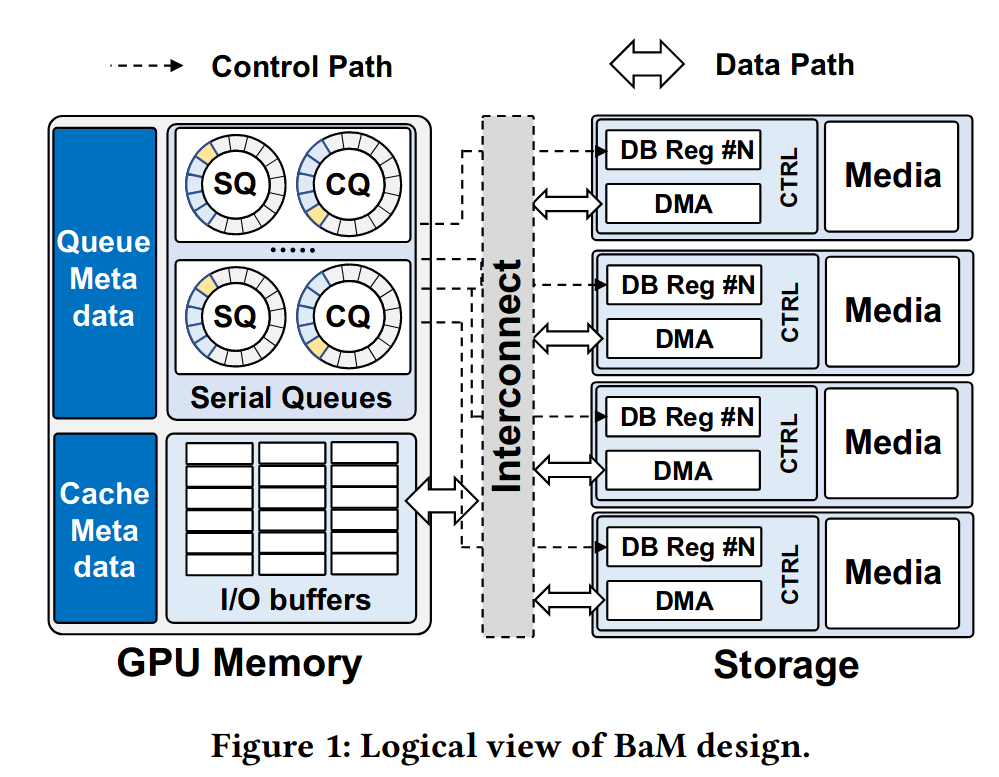
\includegraphics[width=.5\textwidth, height=.5\textheight, keepaspectratio]{images/bam.png}
  \end{figure}
\end{frame}

\subsection{3.2 BaM Workflow}\label{sec:3-2}
\begin{frame}[t]
  \frametitle{3.2 BaM 工作流程}
    \begin{wrapfigure}[8]{r}{15.5em}
      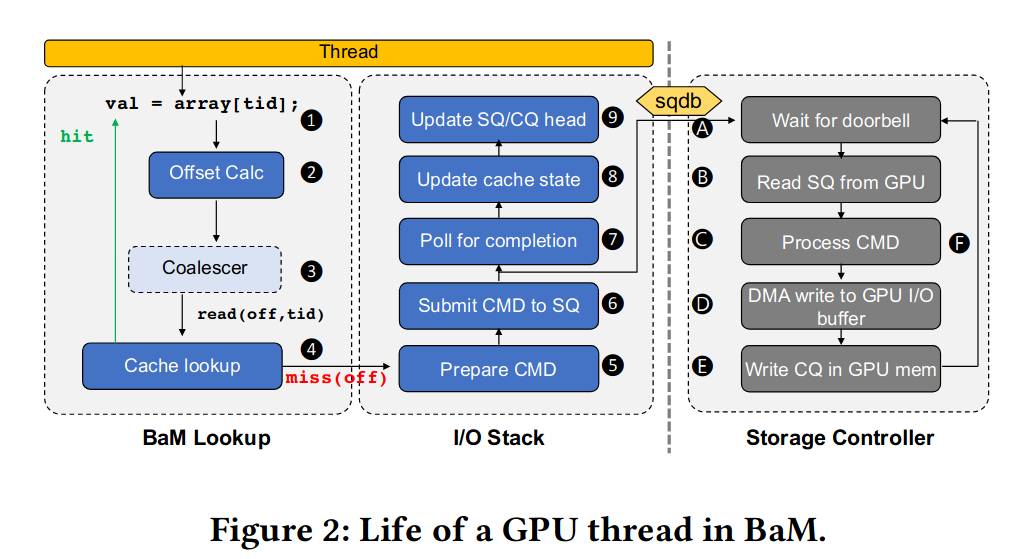
\includegraphics[width=.5\textwidth, height=.5\textheight, keepaspectratio]{images/bam-workflow.png}
    \end{wrapfigure}
    \begin{minipage}{0.5\textwidth}
      BaM的工作流程:
      \begin{enumerate}
        \item GPU线程通过BaM::array来访问数据
        \item BaM系统通过array的偏移来计算文件对应的偏移
        \item coalescer合并同一个warp中的GPU线程的访问
        \item 如果访问的是相同的cacheline,只有一个线程进行访问
        \item 如果cacheline无数据,就会准备IO命令
        \item 向SQ中提交IO命令
        \item 等待SSD完成IO命令
        \item 更新BaM的cacheline
        \item 更新SQ和CQ的头
      \end{enumerate}      
    \end{minipage}
\end{frame}

\subsection{3.3 BaM Design}\label{sec:3-3}
\begin{frame}[t]
  \frametitle{3.3 BaM 设计}
  \framesubtitle{High-Throughput I/O Queues}
  原本的SQ和CQ队列是由CPU维护的,不适用于高度并发的GPU访问。BaM设计了一个高度并发的提交/完成协议队列库,用于GPU线程提交和完成IO命令。
  BaM 在 GPU 内存中保留每个 SQ 的以下元数据
  \begin{enumerate}
    \item SQ的head和tail的本地副本
    \item 原子计数器,ticket
    \item turn\_counter数组,长度与SQ队列长度相同
    \item mark标记位,向量长度与SQ队列长度相同
    \item lock,锁
  \end{enumerate}

\end{frame}

\begin{frame}
  当GPU线程想要将命令放入SQ时
  \begin{enumerate}
    \item 将SQ的ticket自增加2返回,根据ticket值分配SQ的物理条目以及轮次turn
    \begin{itemize}
      \item $ entry = ticket \mod length_{SQ} $
      \item $ turn = ticket/length_{SQ} $
    \end{itemize}
    \item 轮旬turn\_counter[entry]的值,直到turn=turn\_counter[entry]
    \item 调用`move\_tail'来移动SQ的tail:获取锁,并将mark[entry]置为1
    \begin{itemize}
      \item 如果其他的线程想读取同一块区域,会因为读取到mark[entry]为1而直接返回
    \end{itemize}

  \end{enumerate}
  
\end{frame}

\begin{frame}
  提交线程的命令后,线程可以在没有任何锁定的情况下轮询CQ,以查找其提交的请求的完成条目。
  \begin{itemize}
    \item 当它找到完成条目时,它会通过 CQ 标记位向量中 CQ 头的下一个移动来标记要出队的条目。
    \item CQ 的头部和门铃的管理方式与 SQ 的尾部类似,获取锁,mark[entry]置1,但是如果发现该条目已经出列会停止尝试。
    \item 获取锁的线程会写DB响门铃来告知SSD已经完成读取。
  \end{itemize}
  存储控制器通过在每个 CQ 条目中指定新的 SQ 头来传达转发进度。
  \begin{itemize}
    \item  具有CQ锁的线程从标记位被其重置的最后一个CQ条目中读取entry
    \item   ,然后从当前SQ头迭代直到指定的新头,将每个位置的turn\_counter值增加1(到偶数值),允许等待这些位置的线程将其命令排队。
    \item   然后线程更新SQ头并释放CQ锁
  \end{itemize}
\end{frame}

\begin{frame}
  \frametitle{BaM Software Cache}
  BaM提供了一个高吞吐量且可扩展的软件定义缓存和相应的API,来提高对局部性的利用。
  \begin{itemize}
    \item 为了优化对大小受限的GPU内存利用和存储带宽
    \item 旨在减少不必要的I/O请求,如果访问的内容不在cacheline,锁定cacheline,然后发出I/O请求
    \item 使用了 clock replacement算法,当cacheline满时,替换最久未使用的cacheline
    \item Warp coalescing 
    \begin{itemize}
      \item threads decide on a leader and only the leader queries the cache and manipulates the requested cachline's state.
    \end{itemize}
  \end{itemize}
\end{frame}


\section[4.Evaluation]{4.Evaluation}\label{sec:4}

\begin{frame}
  \frametitle{4.Evaluation}
  \framesubtitle{BaM Prototype System}
  \begin{itemize}
    \item 定制化驱动
    \begin{itemize}
      \item 利用 GPUDirect RDMA API 来固定和映射NVMe 队列和 I/O 缓冲区到GPU内存中。
      \item 利用 GPUDirect Async将 NVMe SSD 门铃(DB寄存器)映射到 CUDA 地址空间,以便 GPU 线程可以按需写Doorbell register。
    \end{itemize}
    \item 硬件配置
  \end{itemize}
  \begin{figure}
    \centering
    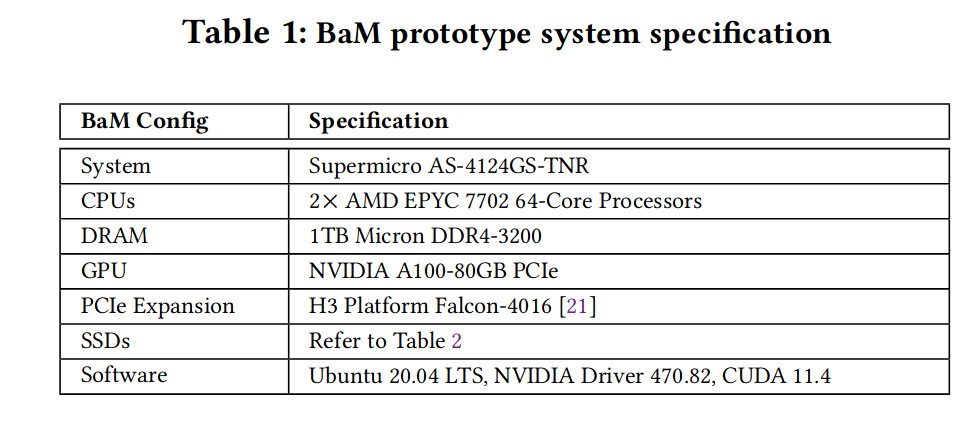
\includegraphics[width=.5\textwidth, height=.5\textheight, keepaspectratio]{images/systab.png}
    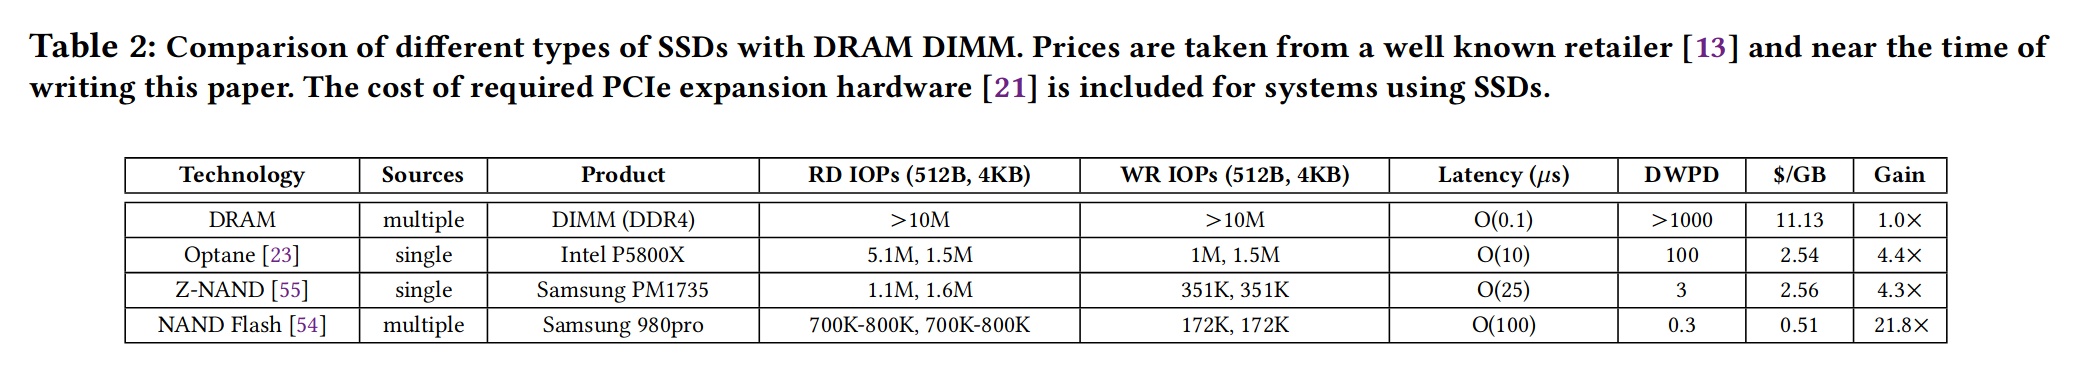
\includegraphics[width=.8\textwidth, height=.4\textheight, keepaspectratio]{images/SSD.png}
  \end{figure}
\end{frame}

\begin{frame}
  \frametitle{4.Evaluation}
  \framesubtitle{Raw Throughput}
  通过使用 Intel Optane SSD 和 NVIDIA A100 GPU 的微基准测试来测量 BaM 的原始吞吐量,可以确定BaM可以生成足够的I/O请求以使底层存储系统饱和。
  
  \begin{figure}
    \centering
    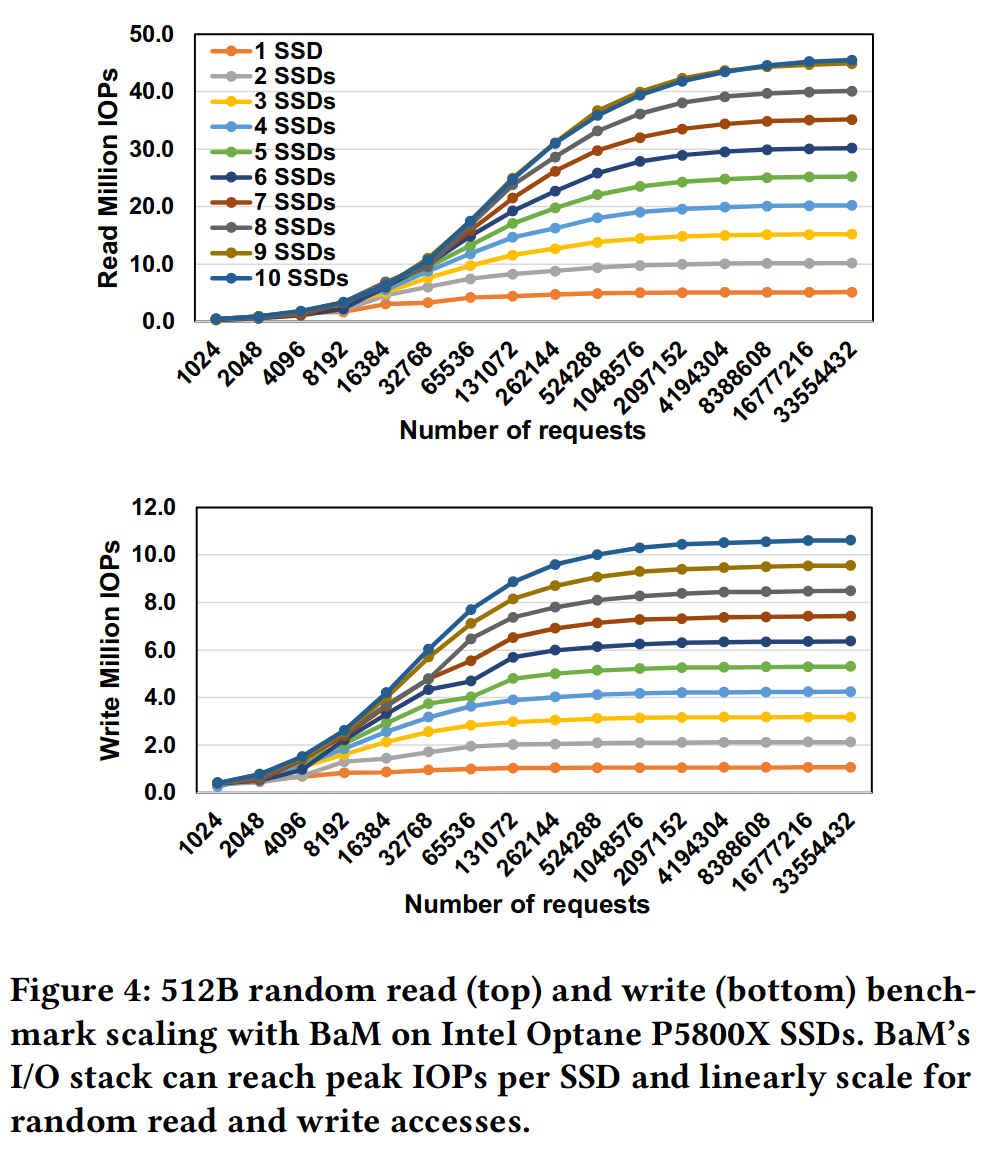
\includegraphics[width=.5\textwidth, height=.8\textheight, keepaspectratio]{images/iops.png}
  \end{figure}
\end{frame}


\begin{frame}
  \frametitle{4.Evaluation}
  \framesubtitle{Compare with GDS}
  GDS(GPUDirect Storage)是NVIDIA通过DMA引擎使得GPU与SSD块设备直接数据传输的技术。\
  实验比较了对于不同I/O块大小,对于16路PCIe带宽的利用率(同时连接4个SSD)。
  \begin{itemize}
    \item 对于GDS,使用fio将128GB数据从4个SSD搬运到GPU内存中
    \item 对于BaM,每个warp分配一个cacheline,大小和I/O块大小相同,连续访问128GB的数据集
  \end{itemize}
  \begin{figure}
    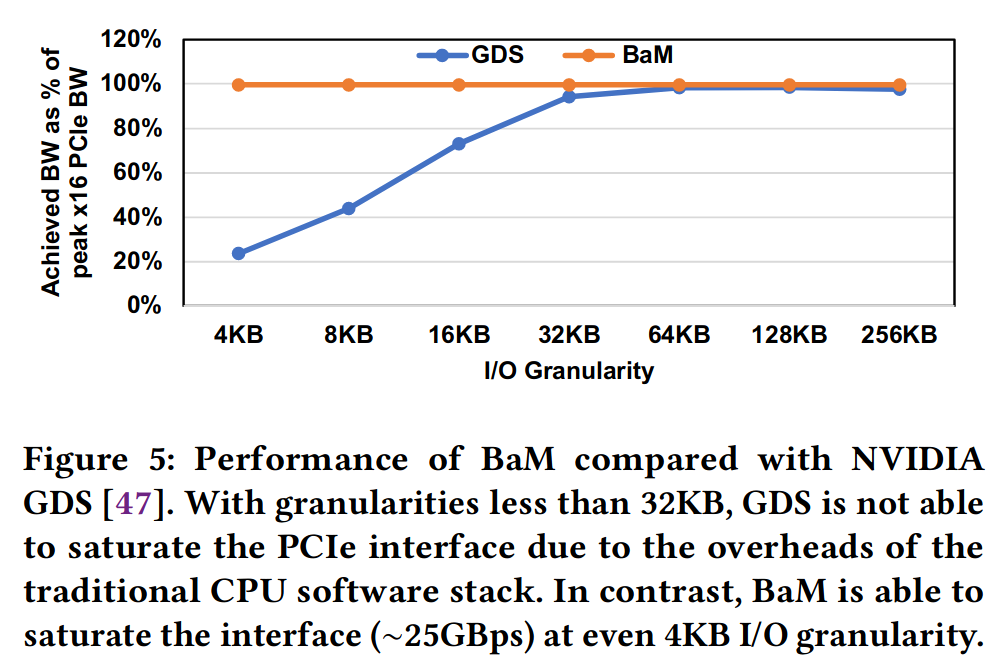
\includegraphics[width=.4\textwidth,height=.4\textheight]{images/gds.png}
  \end{figure}

\end{frame}

\begin{frame}
  \framesubtitle{performance benefit over graph analytics}
  BaM 的目标是提供与基于主机内存的 DRAM 图形分析解决方案相比具有竞争力的性能。
  \begin{itemize}
    \item 基准对比对象:EMOGI,允许 GPU 线程直接对存储在主机内存中的图数据执行合并细粒度访问 \cite{min2020emogi}。
    \item 实验数据集:从the SuiteSparse Matrix collection选取了最大的4个图数据集(K,U,F,M),
    \item 图算法:BFS和CC(计算连通分量)
  \end{itemize}
  \begin{figure}
    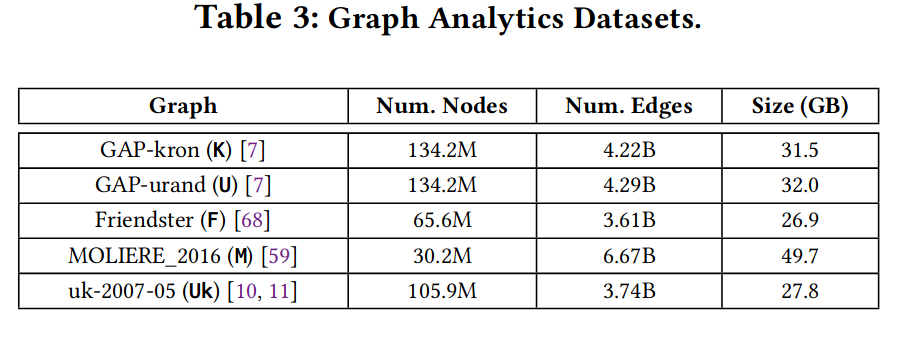
\includegraphics[width=.3\textwidth,height=.2\textheight]{images/dataset.png}
    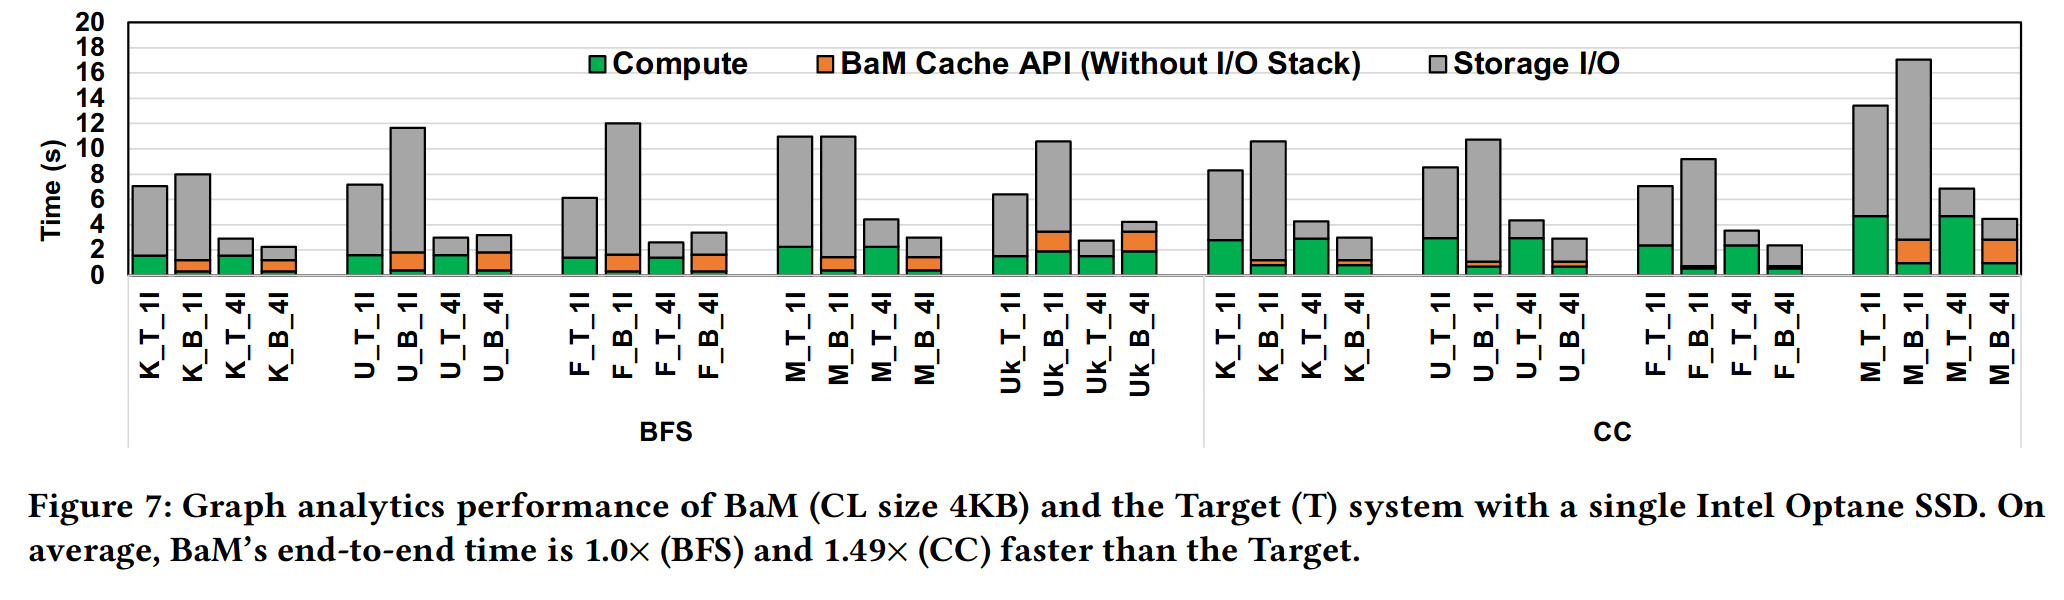
\includegraphics[width=.65\textwidth,height=.3\textheight]{images/graph_analysics.png}
  \end{figure}
  % \blfootnote{
  %   \printbibliography[heading=none,keyword=emogi,]
  % }

\end{frame}

\begin{frame}
  \frametitle{4.Evaluation}
  \framesubtitle{Impact of SSD type}
  作者不仅适用了Intel Optane SSD测试,还使用性能不同的Samsung S980PRO和Samsung Datacenter S1735进行对比测试。
  \begin{itemize}
    \item 测试环境:使用对应型号的4块SSD进行测试,以利用PCIe x16的带宽
  \end{itemize}
  \begin{figure}
    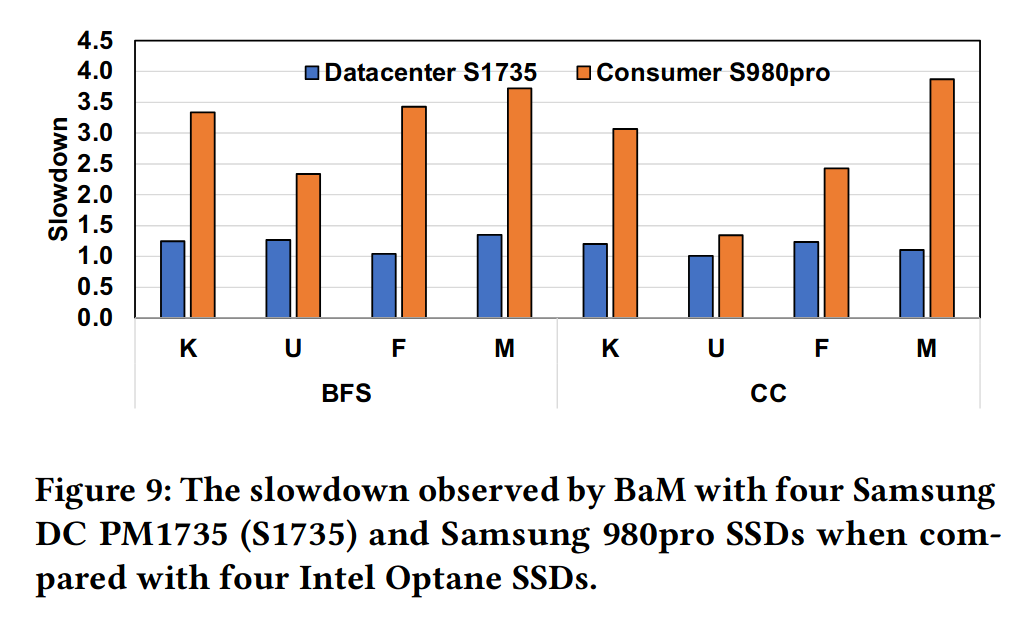
\includegraphics[width=.5\textwidth,height=.5\textheight]{images/ssd-type.png}
  \end{figure}

\end{frame}
\begin{frame}
  \frametitle{4.Evaluation}
  \framesubtitle{Drawbacks in VectorAdd Workload}
  VectorAdd Workload实验:测试BaM在写密集型的工作负载情况\
  \begin{itemize}
    \item vectorAdd工作负载需要两个输入数组,每个数组包含 40 亿个元素,其中每个元素的大小为 8 字节。数据都存储在SSD中,进行加法操作后写回SSD
    \item 基准对比对象:we use a proactive tiling approach and split the four billion elements into five tiles
  \end{itemize}
  \begin{itemize}
    \item 结果:BaM比基准对象慢了1.51倍
    \item 原因:BaM目前不支持read miss和write-back 时间上的重叠。(我猜测是cache起不到作用了)
  \end{itemize}
\end{frame}
\begin{frame}[noframenumbering, allowframebreaks, t]
  \frametitle{参考文献}
  \nocite{*}% 打印未引用,但已列入 .bib 文件内的文献
  \printbibliography%
\end{frame}

\begin{frame}[plain]
  \vfill
  \centerline{\Huge 谢谢}
  \vfill
\end{frame}

\end{document}

